\documentclass{article}[12pt]

\usepackage[utf8]{inputenc}
\usepackage{amsfonts,amssymb,amsmath,subfigure}
\usepackage[pdftex]{graphicx}
\usepackage{epstopdf}
\usepackage{vmargin}
\usepackage{comment}
\usepackage{tikz,multicol}

\usepackage{algorithm}
\usepackage[noend]{algpseudocode}
\usepackage{tcolorbox}

\newtcolorbox{mybox}[3][]
{
  colframe = #2!25,
  colback  = #2!10,
  coltitle = #2!20!black,  
  title    = {#3},
  #1,
}


\newcommand*\Let[2]{\State #1 $\gets$ #2}
\algrenewcommand\algorithmicrequire{\textbf{Precondition:}}
\algrenewcommand\algorithmicensure{\textbf{Postcondition:}}




\excludecomment{solution}
%\includecomment{solution}

\title{IF111 - Algorithmes et structures de données\\EI4 - ABR et Graphes}
\date{\texttt{rfosse@labri.fr}}
\author{Rohan Fossé}
\begin{document}



\maketitle{}


\section*{Recherche dans un ABR}
\begin{enumerate}
    \item Écrire une fonction qui retourne $true$ si l’ABR qui lui est passé en paramètre
est une feuille.
    \item  Écrire une fonction récursive qui affiche l’ABR qui lui est passé en paramètre, par ordre croissant des valeurs.
    \item Écrire une fonction récursive qui affiche l’ABR qui lui est passé en paramètre, par ordre décroissant des valeurs.
    \item Écrire une fonction qui retourne la hauteur de l’ABR qui lui est passé en
paramètre.
\item Écrire une fonction qui retourne le nombre de nœuds de l’ABR qui lui est
passé en paramètre.
\end{enumerate}

\begin{figure}[hbtp] 
  \centering
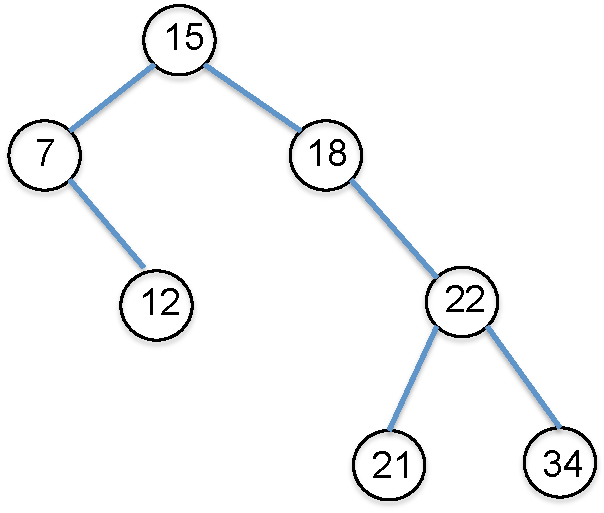
\includegraphics[scale =0.5] {ABR.pdf}\label{fig:abr} \caption{Arbre binaire de recherche}
\end{figure}

\section*{Suppression dans un arbre binaire de recherche}
Soit l’arbre binaire de recherche donné dans la figure 1
\begin{enumerate}
    \item Dessiner l’arbre après la suppression du noeud 18.
    \item  L’opération suppression est-elle ”commutative” au sens où la suppression de x puis de y dans un arbre binaire de recherche produit le même arbre que la suppression de y puis
de x.\\
Si oui dire pourquoi, sinon donner un contre exemple.
\end{enumerate}



\newpage

\section*{Algorithme de Dijkstra}
On considère maintenant des graphes pondérés. Appliquer l'algorithme de Dijkstra au graphe dans la Figure \ref{fig:grapheDijkstra} pour calculer la plus courte distance de $B$ à $D$.

\begin{figure}[h!] 
  \centering
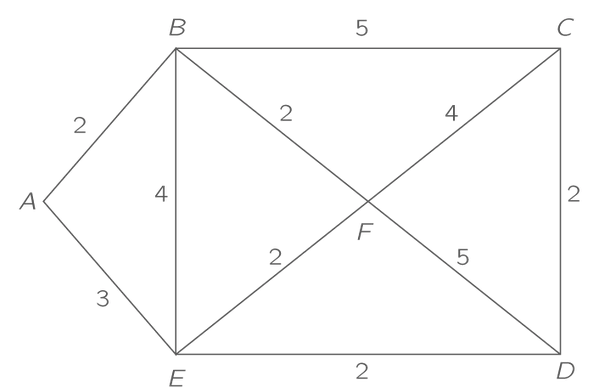
\includegraphics[scale =0.3]{Djikstra.png}
\caption{Graphe pour Dijkstra.} \label{fig:grapheDijkstra}
\end{figure}

\section*{Récursivité sur les arbres}
\begin{enumerate}
\item Dessiner l'arborescence binaire ayant 10 noeuds \{0, 1, 2, ..., 9\}, telle que le parcours infixe et le parcours postfixe de cette arborescence produisent respectivement les suites suivantes : 9, 3, 1, 0, 4, 2, 6, 7, 8, 5 (infixe) et 9, 1, 4, 0, 3, 6, 7, 5, 8, 2 (postfixe). Dire quel est le raisonnement utilisé pour arriver à la solution.\\ Dire quelle est la hauteur du noeud 1 et 2 dans l'arborescence dessinée et quelle est la hauteur de l'arborescence elle même. \\

\end{enumerate}

\section*{Coloration de graphes}

\begin{figure}[h!]
    \centering
    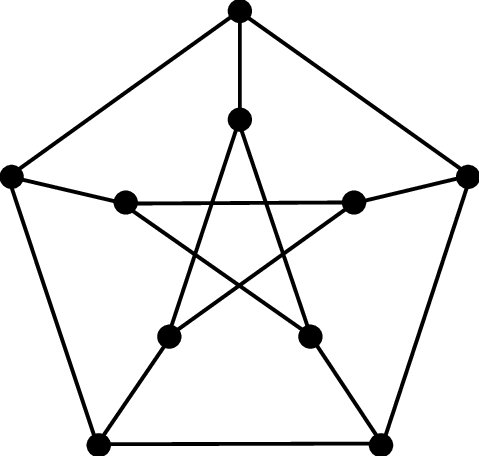
\includegraphics[scale=0.25]{Petersen.png}
    \caption{Graphe de Petersen}
    \label{fig:petersen}
\end{figure}
\begin{itemize}
    \item On cherche à colorier le graphe de la figure \ref{fig:petersen} en utilisant des entiers positifs de façon telle que deux sommets voisins ont des couleurs dont la différence, en valeur absolue, est au moins égale à trois.
    \item Maintenant, on souhaite que, de plus, deux sommets à distance deux aient des couleurs dont la différence, en valeur absolue, est au moins égale à deux. Quelle est la meilleure coloration possible de ce graphe ?

\end{itemize}


\newpage

\section*{La bibliothèque}

Sept élèves, désignés par A,B,C,D,E,F et G se sont rendus à la bibliothèque aujourd'hui. Le tableau suivant précise "qui a rencontré qui" (la bibliothèque étant petite, deux élèves présents au même moment se rencontrent nécessairement…). 

\begin{table}[h!]
\centering
\begin{tabular}{|c|c|c|l|l|l|l|l|}
\hline
\textbf{élève}       & \textbf{A} & \textbf{B} & \textbf{C} & \textbf{D} & \textbf{E}  & \textbf{F} & \textbf{G} \\ \hline
\textbf{a rencontré} & D,E        & D,E,F,G    & E,G        & A,B,E      & A,B,C,D,F,G & B,E,G      & B,C,E,F    \\ \hline
\end{tabular}
\end{table}

De combien de places assises doit disposer la bibliothèque pour que chacun ait pu travailler correctement au cours de cette journée ?

\section*{Degré de graphe}

On s’intéresse aux graphes dont tous les sommets sont de degré trois.
\begin{enumerate}
    \item Construisez de tels graphes ayant 4 sommets, 5 , 6 , 7 .
    \item Qu'en déduisez-vous ?
    \item Prouvez-le !
\end{enumerate}



\section*{Graphes Eulériens}

Soit G un graphe non Eulérien. Est-il toujours possible de rendre G Eulérien en lui rajoutant un sommet et quelques arêtes ?


\section*{Les dominos}

On considère des dominos dont les faces sont numérotées 1, 2, 3, 4 ou 5.

\begin{enumerate}
    \item En excluant les dominos doubles, de combien de dominos dispose-t-on ?
    \item Montrez que l’on peut arranger ces dominos de façon à former une boucle fermée (en utilisant la règle habituelle de contact entre les dominos).
    \item Pourquoi n’est-il pas nécessaire de considérer les dominos doubles ?
    \item Si l’on prend maintenant des dominos dont les faces sont numérotées de 1 à n, est-il possible de les arranger de façon à former une boucle fermée ?
\end{enumerate}


\section*{Les tournois}

Un tournoi est un graphe orienté tel que toute paire de sommets est reliée par un arc, dans un sens ou dans l’autre (mais pas dans les deux sens).

\begin{enumerate}
    \item Pourquoi, selon vous, appelle-t-on de tels graphes des tournois ?
    \item Montrez que si un tournoi contient un circuit de longueur k, alors il contient également des circuits de longueur k', pour tout k' < k (une " preuve " à l’aide d’un dessin suffit…).
    \item Dessinez un tournoi à 6 sommets ne possédant pas de circuit de longueur 4.
\end{enumerate}

\section*{Le robot}
Un robot se promène sur le graphe \ref{fig:robot}. Partant d’un sommet quelconque s, appelé sommet de stockage, il doit déposer un cube sur chacun des autres sommets. Il possède suffisamment de cubes sur le sommet de stockage, mais ne peut transporter qu'un cube à la fois (il doit donc repasser par le sommet de stockage avant de livrer un autre cube).
\begin{enumerate}
    \item Calculer, pour chacun des sommets du graphe, le trajet minimum que doit parcourir le robot si ce sommet est sommet de stockage.
    \item Quel est le "meilleur" sommet de stockage ?
\end{enumerate}

\begin{figure}[h!]
    \centering
    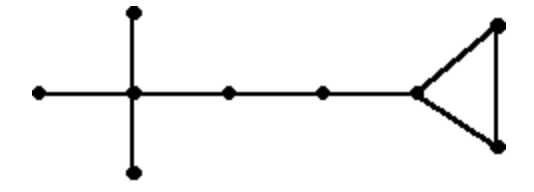
\includegraphics{Robot.png}
    \caption{Graphe du robot}
    \label{fig:robot}
\end{figure}

\section*{Nombres premiers}

Construire le graphe orienté dont les sommets sont les entiers compris entre 1 et 24 et dont les arcs relient x à y lorsque x divise y. De plus, les arcs sont valués par le quotient $\frac{y}{x}$ (ainsi, l’arc allant de 3 vers 15 a la valeur 5).

\begin{enumerate}
    \item Comment reconnaît-on dans ce graphe un nombre premier ?
    \item Comment retrouver dans ce graphe la décomposition d’un nombre en facteurs premiers ?
\end{enumerate}


\end{document}